\documentclass[12pt]{article}
\usepackage[margin=1in]{geometry}
\usepackage{setspace}
\usepackage{amsmath,amssymb}
\usepackage{booktabs}
\usepackage{array}
\usepackage{tikz}
\usepackage{hyperref}
\usepackage{cite}
\usetikzlibrary{arrows.meta,positioning,fit}

\onehalfspacing
\newcommand{\modelname}{A$^2$SNN}

\title{\textbf{Project Proposal}\\[4pt]
Hardware-Aware Lightweight Spiking Neural Network with Adaptive Event-Driven Inference for Resource-Constrained Microcontrollers}
\author{Author Name\\Department Name\\University Name}
\date{2026}

\begin{document}
\maketitle

\begin{abstract}
This project proposes \modelname, an adaptive asynchronous spiking neural network co-designed for resource-constrained microcontrollers. The work addresses a practical gap in edge intelligence: many efficient SNN demonstrations assume FPGA, GPU, or neuromorphic hardware, while low-cost microcontrollers face a different constraint profile dominated by limited SRAM, flash access, sequential instruction execution, and energy budget. The proposed system combines adaptive spike encoding, integer leaky-integrate-and-fire dynamics, sparse event scheduling, and confidence-aware early exit. The expected outcome is a reproducible model and firmware prototype that reports accuracy, memory footprint, latency, cycle count, power, and energy per inference on locally available microcontroller hardware.
\end{abstract}

\section{Background and Motivation}
Machine learning at the edge is increasingly important for low-power sensing, robotics, agriculture, health monitoring, education, and small autonomous systems. In many of these applications, cloud inference is undesirable because of latency, connectivity, privacy, or energy constraints. Microcontrollers are attractive deployment targets because they are inexpensive and widely available, but they impose strict limits on memory and computation.

Spiking neural networks are a promising candidate for low-power inference because their computation is event-driven. Unlike dense neural networks, an SNN can avoid unnecessary synaptic operations when spikes are sparse. However, this advantage is not automatic. If an SNN is implemented with dense layer loops on a microcontroller, much of the event-driven benefit is lost. Therefore, the model architecture and inference engine must be designed together.

This project focuses on a microcontroller-oriented SNN design rather than copying an FPGA-oriented accelerator architecture. FPGA designs can exploit parallel logic and custom datapaths. A commodity MCU must instead manage flash bandwidth, SRAM footprint, integer arithmetic, event queues, and cycle count. This difference motivates the proposed hardware-aware co-design.

\section{Problem Statement}
Existing SNN accelerators often target FPGA or neuromorphic platforms, where hardware parallelism and specialized memory structures can be assumed. Directly transferring these ideas to a commodity MCU is insufficient because MCU inference is constrained by:
\begin{itemize}
    \item small SRAM for membrane states, spike queues, and buffers;
    \item limited flash bandwidth for weight access;
    \item sequential CPU execution and instruction-cycle limits;
    \item lack of efficient floating-point support on many low-cost boards;
    \item power measurement and energy constraints in battery-powered use cases.
\end{itemize}

The research problem is therefore:
\begin{quote}
How can an SNN model and inference engine be jointly designed so that spike activity, numerical precision, memory layout, and inference duration are optimized for microcontroller deployment?
\end{quote}

\section{Research Objectives}
The project has the following objectives:
\begin{enumerate}
    \item Design an adaptive spike encoder that reduces unnecessary input events.
    \item Implement a quantized LIF neuron model using INT8 weights and integer membrane states.
    \item Develop a sparse event-driven inference scheduler for MCU execution.
    \item Add confidence-aware early exit to reduce average inference timesteps.
    \item Deploy the model on ESP32-S3 class hardware and optionally compare with an ARM Cortex-M board.
    \item Measure accuracy, flash usage, peak SRAM, latency, cycles, spike count, power, and energy.
    \item Compare the full system against ANN, fixed-duration SNN, INT8 SNN, and sparse SNN baselines.
\end{enumerate}

\section{Proposed Contribution}
The intended contributions are:
\begin{itemize}
    \item an MCU-aware SNN model architecture named \modelname;
    \item a multiplier-free integer LIF inference formulation;
    \item an event-driven sparse MCU scheduling method;
    \item a confidence-aware early-exit mechanism for adaptive inference duration;
    \item a Bangladesh-marketplace-feasible hardware evaluation plan;
    \item a reproducible thesis and paper-ready experimental methodology.
\end{itemize}

\section{System Architecture}
\subsection{Model Architecture}
The model-level architecture is shown in Fig.~\ref{fig:proposal_model}. The input is preprocessed, encoded into adaptive spike events, processed by a quantized sparse SNN core, and classified through an early-exit readout.

\begin{figure}[h]
\centering
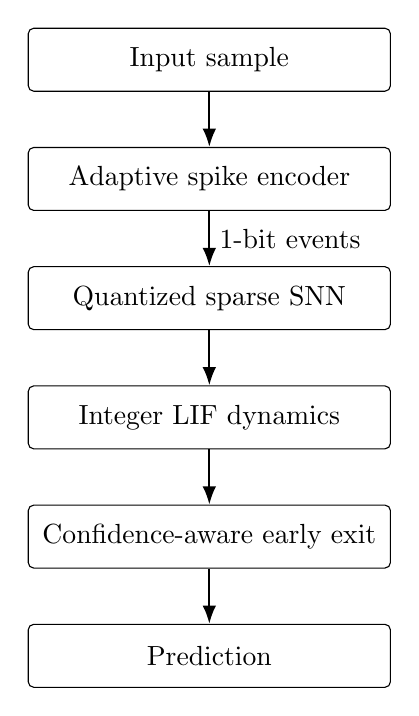
\begin{tikzpicture}[
    node distance=7mm,
    block/.style={draw, rounded corners=2pt, align=center, minimum width=46mm, minimum height=8mm},
    arrow/.style={-Latex, thick}
]
\node[block] (input) {Input sample};
\node[block, below=of input] (enc) {Adaptive spike encoder};
\node[block, below=of enc] (snn) {Quantized sparse SNN};
\node[block, below=of snn] (lif) {Integer LIF dynamics};
\node[block, below=of lif] (exit) {Confidence-aware early exit};
\node[block, below=of exit] (pred) {Prediction};
\draw[arrow] (input) -- (enc);
\draw[arrow] (enc) -- node[right]{1-bit events} (snn);
\draw[arrow] (snn) -- (lif);
\draw[arrow] (lif) -- (exit);
\draw[arrow] (exit) -- (pred);
\end{tikzpicture}
\caption{Proposed \modelname{} model architecture.}
\label{fig:proposal_model}
\end{figure}

\subsection{Hardware Architecture}
The hardware execution architecture is shown in Fig.~\ref{fig:proposal_hardware}. Weights and layer metadata are stored in flash. Membrane states, active event queues, touched-neuron flags, and output counters are stored in SRAM. Timing is measured using GPIO pulses and a logic analyzer when available.

\begin{figure}[h]
\centering
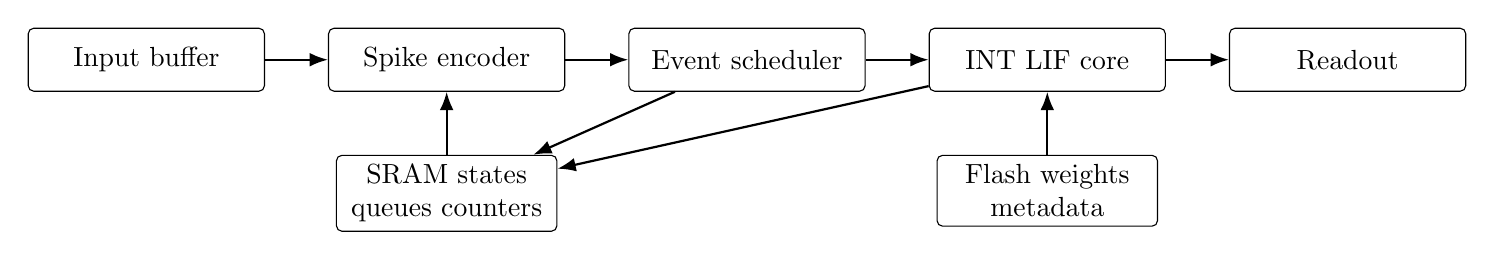
\begin{tikzpicture}[
    node distance=8mm and 8mm,
    block/.style={draw, rounded corners=2pt, align=center, minimum width=30mm, minimum height=8mm},
    mem/.style={draw, rounded corners=2pt, align=center, minimum width=28mm, minimum height=8mm},
    arrow/.style={-Latex, thick}
]
\node[block] (sensor) {Input buffer};
\node[block, right=of sensor] (encoder) {Spike encoder};
\node[block, right=of encoder] (scheduler) {Event scheduler};
\node[block, right=of scheduler] (lif) {INT LIF core};
\node[block, right=of lif] (readout) {Readout};
\node[mem, below=of encoder] (sram) {SRAM states\\queues counters};
\node[mem, below=of lif] (flash) {Flash weights\\metadata};
\draw[arrow] (sensor) -- (encoder);
\draw[arrow] (encoder) -- (scheduler);
\draw[arrow] (scheduler) -- (lif);
\draw[arrow] (lif) -- (readout);
\draw[arrow] (sram) -- (encoder);
\draw[arrow] (scheduler) -- (sram);
\draw[arrow] (flash) -- (lif);
\draw[arrow] (lif) -- (sram);
\end{tikzpicture}
\caption{Microcontroller hardware execution architecture.}
\label{fig:proposal_hardware}
\end{figure}

\section{Mathematical Formulation}
For input $x_i$, an adaptive encoder generates spike $z_i[t]$:
\begin{equation}
    z_i[t] = \mathbb{I}\left(q(x_i) + \eta_i[t] > \tau(a(x))\right),
\end{equation}
where $q(\cdot)$ is integer quantization, $\eta_i[t]$ is temporal dither, and $\tau(a(x))$ is an activity-aware threshold.

The LIF update is:
\begin{equation}
    V_j[t+1] = V_j[t] - (V_j[t] \gg k) + \sum_{i \in \mathcal{A}_t} w_{ij} - \Theta s_j[t].
\end{equation}
Here $w_{ij}$ is INT8, $V_j$ is INT16 or INT32, and $\mathcal{A}_t$ is the active spike set.

Early exit is triggered when:
\begin{equation}
    S_{\max}[t] - S_{\mathrm{second}}[t] > \delta(t),
\end{equation}
where $S_{\max}$ is the highest class score and $S_{\mathrm{second}}$ is the second-highest score.

\section{Methodology}
\subsection{Model Development}
The first stage will implement and train a compact ANN and a fixed-duration SNN baseline. The SNN will then be modified with quantization-aware constraints, integer LIF dynamics, adaptive encoding, and early exit.

\subsection{Firmware Development}
The second stage will implement the MCU inference engine. The firmware will include flash-resident weights, SRAM-resident states, sparse event queues, timing hooks, and serial logging.

\subsection{Hardware Measurement}
Latency will be measured using firmware timers and preferably GPIO pulse timing with a logic analyzer. Power will be measured at board level using INA219 and a USB power meter or better power logger. Energy will be computed as:
\begin{equation}
    E_{\mathrm{inf}} = P_{\mathrm{avg}} \times L_{\mathrm{inf}}.
\end{equation}

\section{Experimental Plan}
\begin{table}[h]
\centering
\caption{Evaluation metrics}
\begin{tabular}{ll}
\toprule
Metric & Unit \\
\midrule
Accuracy & percent \\
Flash usage & KB \\
Peak SRAM & KB \\
Latency & ms/sample \\
Average timestep count & timestep/sample \\
Spike count & spikes/sample \\
CPU cycles & cycles/sample \\
Power & mW \\
Energy & mJ/inference \\
\bottomrule
\end{tabular}
\end{table}

\begin{table}[h]
\centering
\caption{Ablation plan}
\begin{tabular}{ll}
\toprule
Experiment & Purpose \\
\midrule
Compact ANN & Dense baseline \\
Fixed SNN & Standard SNN baseline \\
INT8 SNN & Effect of quantization \\
INT8 + sparse scheduling & Effect of event-driven execution \\
INT8 + sparse + early exit & Effect of adaptive inference duration \\
Full \modelname & Complete proposed system \\
\bottomrule
\end{tabular}
\end{table}

\section{Budget Summary}
The project budget is designed for Bangladesh marketplace availability. A minimum prototype can be built for approximately BDT 2,000--4,500. A balanced thesis setup is expected to cost approximately BDT 8,000--20,000. A fuller lab setup with better measurement equipment, ARM comparison hardware, camera option, and documentation cost is expected to cost approximately BDT 25,000--55,000. If publication-grade energy measurement is required, the budget may increase to approximately BDT 55,000--110,000 depending on the oscilloscope or power profiler used.

\section{Timeline}
\begin{tabular}{p{3cm}p{11cm}}
\toprule
Period & Work package \\
\midrule
Weeks 1--2 & Literature review, dataset choice, final problem framing. \\
Weeks 3--4 & ANN and fixed SNN baseline implementation. \\
Weeks 5--6 & Quantized LIF and adaptive spike encoder. \\
Weeks 7--8 & Sparse event scheduler and early-exit calibration. \\
Weeks 9--10 & MCU firmware implementation and memory optimization. \\
Weeks 11--12 & Hardware measurement: latency, SRAM, flash, cycles, power, energy. \\
Weeks 13--14 & Ablation study, result tables, error analysis. \\
Weeks 15--16 & Final thesis writing, proposal defense updates, paper formatting. \\
\bottomrule
\end{tabular}

\section{Risk Management}
\begin{itemize}
    \item If CIFAR-10 is too heavy for the selected MCU, use MNIST or Fashion-MNIST for hardware validation and keep CIFAR-10 as workstation-level analysis.
    \item If power measurement is noisy, report board-level energy transparently and avoid chip-only claims.
    \item If sparse scheduling overhead exceeds savings, report the crossover point where event-driven execution becomes useful.
    \item If early exit reduces accuracy, calibrate the margin threshold and report the accuracy-latency trade-off.
\end{itemize}

\section{Expected Outcomes}
The expected outcomes are:
\begin{itemize}
    \item a trained lightweight SNN model;
    \item an MCU inference kernel using integer LIF dynamics;
    \item an event-driven sparse scheduler;
    \item a measured hardware evaluation table;
    \item a complete thesis proposal and journal-style manuscript draft.
\end{itemize}

\section{Conclusion}
This project proposes a practical, hardware-aware SNN design for microcontroller inference. The research value lies in aligning the model architecture with MCU bottlenecks: integer arithmetic, flash/SRAM limits, sparse event processing, and adaptive inference duration. The final system is expected to provide a defensible embedded ML prototype and a clear research contribution beyond direct deployment of an existing FPGA-oriented SNN accelerator.

\bibliographystyle{IEEEtran}
\bibliography{references}

\end{document}
